\documentclass[12pt]{article}
\usepackage[margin=1.5cm]{geometry}
\usepackage{parskip}
\usepackage{amsmath}
\usepackage{amssymb}
\usepackage{amsfonts}
\usepackage{enumitem}
\usepackage{graphicx}
\usepackage{stmaryrd}
\graphicspath{ {./images/} }


\begin{document}
\begin{enumerate}[label=(\alph*)]
  \item
    \begin{enumerate}[label=(\roman*)]

      \item
        We create the following alignment:

        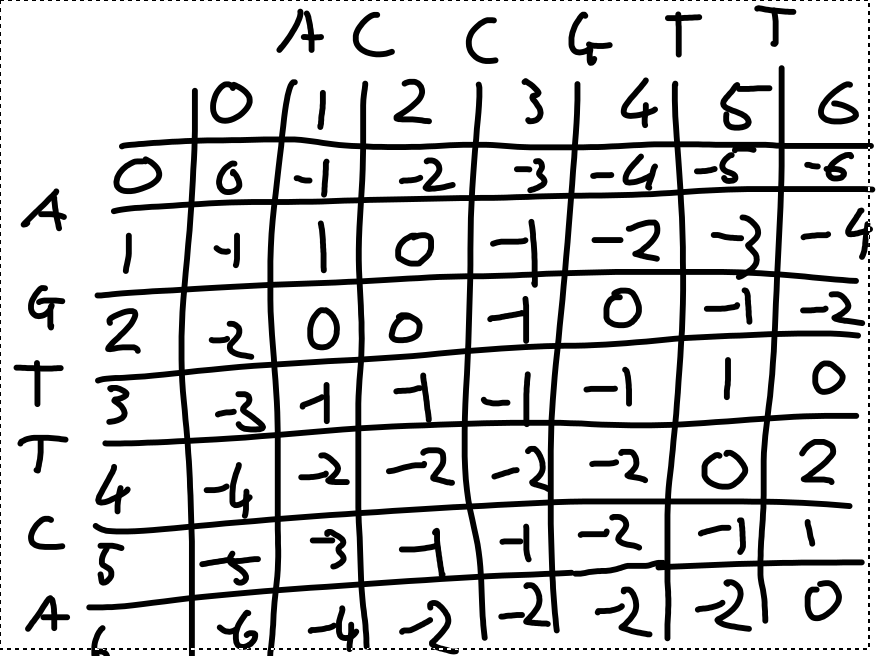
\includegraphics[scale=0.3]{alignment}

        So the maximum similarity score between the two sequences is 0.

      \item

        We give the following alignment:

\begin{verbatim}
ACCGTT--
A--GTTCA
\end{verbatim}

\item
  The alignment is unique, there are no other valid paths through the similarity matrix.

    \end{enumerate}

  \item
    The Sankoff parsimony algorithm works character by character, so we consider only a single character to begin with.

    The Sankoff parsimony algorithm is a dynamic programming algorithm, so to calculate the parsimony vector for a particular internal node, we need to take each possible state in turn, and calculate the parsimony for both the son and daughter. So if we have $k$ different states, then this has $O(k^2)$ complexity. If there are $n$ internal nodes in our tree, then calculating the best parsimony score for a single character takes time $O(nk^2)$.

    Finally, if each leaf is labelled with a string of $m$ characters, then the whole algorithm takes time $O(mnk^2)$.

  \item
    (Superparamagnetic not relevant).

    The $k$-means algorithm is a clustering algorithm that takes in a set of $n$-dimensional points and a positive integer $k$, and forms $k$ clusters for the $n$-dimensional points, that attempts to 
uster the points by similarity.

The Markov clustering algorithm is intended to find a clustering for graphs, not sets of $n$-dimensional points. Furthermore, the Markov clustering algorithm does not require an input that gives the desired number of clusters, instead the algorithm decides on a clustering. It does this by forming an adjacency matrix of the graph and normalising each column to sum to 1. Then, we take the $k$th power (usually 2) to expand the matrix, and raise each element of the matrix by power $r$. These parameters implicitly control the clustering results.

The $k$-means algorithm has complexity $O(n^2)$, whereas the Markov Clustering algorithm does not even have a definite time for convergence, and each iteration takes time $O(n^3)$ (although matrices are usually sparse). So, the flexibility of the Markov Clustering algorithm in not needing to specify a number of clusters comes at the expense of performance.

\item
  The Doob-Gillespie algorithm in system biology is a stochastic algorithm to estimate molecule concentrations in a mixture over time.

  The algorithms works as follows, after setting up a set of reactions $R$ and initial molecule concentrations.

  \begin{itemize}
    \item
      Derive propensities for each of the reactions based on molecule concentrations.

    \item
      Using the normalized propensities as a probability distribution, randomly choose a reaction to occur.

    \item
      Using the aggregate propensity in an exponential distribution, decide on how long the reaction should take place for.

    \item
      Using these two values, calculate new molecule densities according to the reaction and the time, and repeat.
  \end{itemize}

  The algorithm is useful for simulating complex molecular reactions, but relies on the assumptions that molecular reactions always occur in series (which we can reasonably achieve with very small time steps), and that the molecular mixture is well-stirred. As long as these assumptions are reasonable, the algorithm has good utility.

        
\end{enumerate}
\end{document}

